% Document class
\documentclass[10pt]{article}

% Preamble
\usepackage[a4paper,margin=2.5cm,includefoot]{geometry} % includefoot makes footer stay inside of the page
\usepackage{titling}
\usepackage{fancyhdr}
\usepackage[hidelinks]{hyperref}
\usepackage[czech]{babel}
\usepackage{amsthm}
\usepackage{mathtools}
\usepackage{enumitem} % for a,b,c enums
\usepackage{caption}

% FONT SPEC (for XeLaTeX) TO MAKE TROJA PRINTER WORK
\usepackage{fontspec}
\usepackage{unicode-math}

% For coloring solutions
\usepackage{xcolor}

%% metadata settings
\newcommand{\tutnum}{0}
\title{Řešení příkladů z \tutnum. cvika diskrétní matematiky}
\author{Jan Hartman}
\date{29.9.2025}

\newcommand{\teacherurl}{https://kam.mff.cuni.cz/~hartmaj/}
\newcommand{\titlerule}{%
    \noindent %
    \makebox[\textwidth]{\large \thetitle \hfill \thedate}
    \rule{\textwidth}{0.4pt}%
}

% remove default caption by czech babel
\captionsetup[figure]{labelformat=empty}

%% headers and footers settings
\renewcommand{\headrulewidth}{0pt}
\renewcommand{\footrulewidth}{0.4pt}
\pagestyle{fancy}
\fancyhf{} % clear all header/footer (e.g. by default, footer would show page numbers)
% \fancyhead[L]{\thetitle}   % left -> title
% \fancyhead[C]{} % center -> unused
% \fancyhead[R]{\thedate}  % right -> date
\fancyfoot[C]{\small Více info k cvičení: \url{\teacherurl}}  


% theorem styles
\newtheoremstyle{definitionstyle}{10pt}{10pt}{\normalfont}{}{\bfseries}{.}{ }{\thmname{#1}}
\newtheoremstyle{problemstyle}{10pt}{10pt}{\normalfont}{}{\bfseries}{.\newline}{ }{\thmname{#1}\thmnumber{ #2}\thmnote{ (#3)}}

% theorems
\theoremstyle{definitionstyle}
\newtheorem{defn}{Definice}
\theoremstyle{problemstyle}
\newtheorem{problem}{Příklad}

% Document body
\begin{document}

\titlerule

\section{Výroky}

\begin{minipage}{0.7\textwidth}
V následujících příkladech uvažujeme množinu států: $$M = \{ \text{Francie}, \text{Německo}, \text{Česko}, \text{Slovensko} \}$$ a nechť $V(x,y)$ je zkratka pro výrok: „Stát $x$ vyváží víno do státu $y$.“. Vztah $V$ je znázorněn na diagramu vpravo.
\end{minipage}%
\hfill
\begin{minipage}{0.15\textwidth}
  \centering
  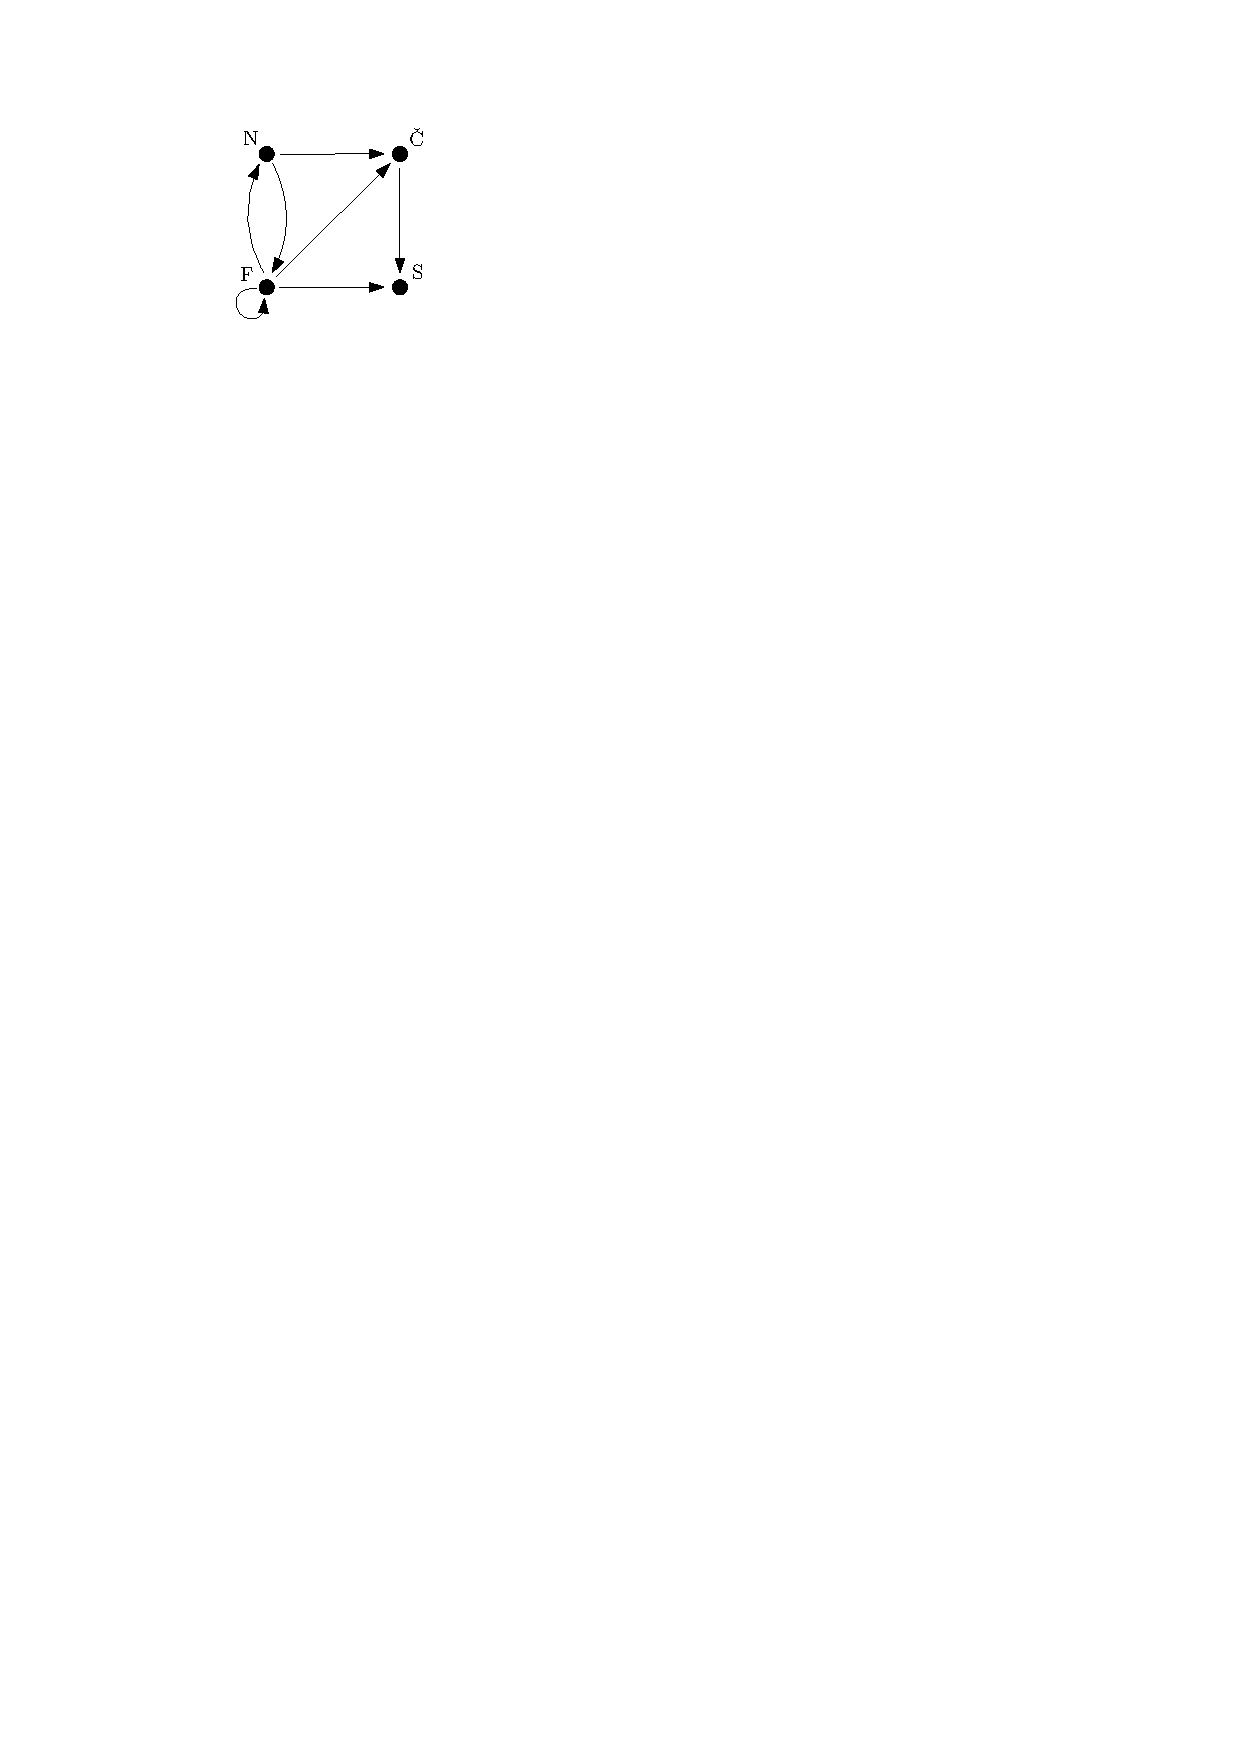
\includegraphics[width=2.2cm]{states.pdf}
\end{minipage}

\begin{problem}[Překládání]
Vyjádřete výroky v přirozeném jazyce matematickými symboly a naopak:
\begin{enumerate}[label=(\alph*)]
    \item \text{Slovensko vyváží víno do Francie.} \textcolor{red}{$V(\text{Slovensko},\text{Francie})$}
    \item $\exists y \in M : V(\text{Německo},y)$ \textcolor{red}{Existuje stát, do kterého Německo vyváží.}
\end{enumerate}
\end{problem}

\begin{problem}[Pořadí kvantifikátorů]
Vyjádřete následující výroky slovy a následně určete, zda jsou pravdivé či lživé:
\begin{enumerate}[label=(\alph*)]
    \item $\forall x \in M \ \exists y \in M : V(x,y)$ 
    \textcolor{red}{Všechny státy někam vyváží. Musí z každé tečky jít šipka ven. To neplatí kvůli Slovensku.}
    \item $\forall x \in M \ \exists y \in M : V(y,x)$
    \textcolor{red}{Do každého státu někdo dováží. Musí vést šipka do každé tečky. To platí.}
    \item $\exists x \in M \ \forall y \in M : V(x,y)$
    \textcolor{red}{Existuje stát, který vyváží do všech států. Musí existovat jedna tečka ze které jdou šipky do všech teček. Pozor, že musí jít šipka i do té tečky samotné. To platí díky Francii.}
    \item $\exists x \in M \ \forall y \in M : V(y,x)$
    \textcolor{red}{Existuje stát, do kterého všechny státy vyváží. Musí existovat jedna tečka do které jdou šipky ze všech teček. To neplatí. Pozor, že i kdyby Německo vyváželo do Slovenska, tak Slovensko výrok stále nesplňuje, jelikož nevyváží samo do sebe.}
\end{enumerate}

\end{problem}

\begin{problem}[Důkazy]
O jisté množině států $E$ jsme zjistili, že splňujě:
\begin{enumerate}
    \item $\forall x \in E \ \forall y \in E: V(x,y) \Rightarrow \neg V(y,x)$
    \item $\forall x \in E \ \forall y \in E \  \forall z \in E : V(x,y) \wedge V(y,z) \Rightarrow V(x,z)$
    % NOTE: Zeptat se a ukázat, co znamená tato tranzitivní podmínka obrázkově.
\end{enumerate} 
\begin{enumerate}[label=(\alph*)]
    \item Zkuste formulovat podmínky vlastními slovy. Splňuje tyto podmínky i množina $M$ zmíněná výše?
    
    \textcolor{red}{První podmínka říká, že když jeden stát vyváží do druhého, tak ten druhý nesmí vyvážet zpět.}
    
    \textcolor{red}{Druhá podmínka znamená, že pro každou trojici států $x,y,z$ platí, že když ten první vyváží do druhého a zároveň ten druhý vyváží do třetího, tak už nutně vyváží ten první do třetího.}
    
    \textcolor{red}{Na šipkách to znamená, že když mezi třemi tečkami nastane situace, kdy se dá z první tečky dostat po dvou šipkách s mezikrokem ve druhé tečce do té třetí, tak nutně musí existovat i šipka rovnou z první tečky do té třetí. Doporučuji nakreslit si obrázek}
    \item Dokažte, že v $E$ neexistuje stát, který vyváží víno sám sobě. 
    % NOTE: Tady jsem se trochu zamotal při vysvětlování. Proč když dosadím za oba kvantifikátory ten samý prvek, tak tabulkou hned vidím, že vyjde 0.
    \textcolor{red}{Dokážeme sporem. Kdyby existoval stát $s$, který vyváží do sebe, tak platí $V(s,s)$. Podmínka jedna však říká, o všech $x,y$ že pokud platí $V(x,y)$, tak nutně neplatí $V(y,x)$. Pokud tedy zvolíme $x=s, y=s$, tak dostaneme spor.}

\end{enumerate}

\end{problem}

\section{Množiny}
% NOTE: Před řešením těchto příkladů nezapomenout zmínit Vennovy diagramy!

\begin{defn}
    Symetrický rozdíl $A \bigtriangleup B$ definujeme jako množinu prvků, které jsou buď v $A$, anebo v $B$ (ale ne v $A$ i $B$ zároveň).
\end{defn}

\begin{problem}[Symetrický rozdíl pomocí ostatních operací]
Zapište množinu $A \bigtriangleup B$ pomocí množinových operací $\cup, \cap, \setminus$. Nemusíte využít všechny uvedené operace. Zkuste najít aspoň dva způsoby.

\textcolor{red}{Jeden způsob je: $A \bigtriangleup B = (A \cup B) \setminus (A \cap B)$}

\textcolor{red}{Druhý způsob je: $A \bigtriangleup B = (A \setminus B) \cup (B \setminus A)$}
\end{problem}

\begin{problem}[Dvouprvkové podmnožiny]
Mějme libovolnou množinu $K$. Uvažme všechny její podmnožiny obsahující právě dva prvky. Jaké množiny jsme z nich schopni vytvořit pomocí operace $\bigtriangleup$? Jsme takto schopni zkonstruovat libovolnou podmnožinu množiny $K$?
% NOTE: Zde nebylo studentům jasné zadání. Bylo by dobré nejprve ukázat konkrétní příklad např. pro čtyřprvkovou množinu.


\textcolor{red}{Nejprve je dobré, představit si nějakou konkrétní množinu. Třeba $K_1 = \{1,2,3\}$. Poté zkusit postupně vytvářet množiny různé velikosti. }

\textcolor{red}{Jaké jsou všechny dvouprvkové podmnožiny množiny $K_1$? To jsou množiny $\{1,2\},\{1,3\},\{2,3\}$, které si pojmenujme $A,B,C$}


\textcolor{red}{Dokáži z množin $A,B,C$ pomocí operace $\bigtriangleup$ sestrojit prázdnou množinu? Dokáží sestrojit nějakou jednoprvkovou množinu? Tříprvkovou?}

\textcolor{red}{Kdyby $K$ měla více než 3 prvky, tak čtyřprvková množina jde vyrobit lehce. No a vlastně i šesti-, osmi- atd. prvkové. Vlastně dokáži vytvořit každou podmnožinu sudé velikosti.}

\textcolor{red}{Jaké množiny nám tedy nejdou vytvořit? Ty liché! Jak ale dokázat, že to tak opravdu je?}

\textcolor{red}{Je užitečné si seřadit a očíslovat prvky množiny $K$ do vektoru $(x_1, \ldots x_n)$. Každou podmnožinu $A \subseteq K$, pak můžeme vyjádřit jako vektor nul a jedniček kde na $i$-té pozici se nachází $1$ právě tehdy když $x_i \in K$.}

\textcolor{red}{Například pro $K_1$ by množina $\{ 1, 3\}$ odpovídala vektoru $(1,0,1)$ nebo zkráceně $101$.}

\textcolor{red}{Co dělá operace $\bigtriangleup$ v jazyku těchto vektorů jedniček a nul? }

\textcolor{red}{Co ta operace $A \bigtriangleup B$ dělá je, že provede operaci XOR na odpovídajících si pozicích ve vektorech množin $A$ a $B$. S tím že tabulka pro XOR je:}

\textcolor{red}{
\begin{tabular}{|c|c|c|}
\hline
$a$ & $b$ & $\oplus$ \\
\hline
0 & 0 & 0 \\
0 & 1 & 1 \\
1 & 0 & 1 \\
1 & 1 & 0 \\
\hline
\end{tabular}
}

\textcolor{red}{Co nás zajímá je, jaký počet jedniček bude obsažen ve výsledném vektoru množiny $A \bigtriangleup B$? Důležité je, že o vektorech množin $A$ a $B$ víme, že obsahují sudý počet jedniček.}

\textcolor{red}{Počítejme výsledné jedničky následovně: Nejprve spočítáme kolik jich může být potenciálně, kdyby se žádné nevykrátily. Sečtu počet jedniček ve vektorech množin $A$ a $B$ a označím toto číslo $k$. Číslo $k$ je nutně sudé číslo, jelikož vzniklo jako součet dvou sudých čísel. To jsme se ale přepočítali a musíme z výsledné sumy odečíst ty vykrácené jedničky. Ty se však pro každý index zkrátí obě (tedy jeden pár pro každý index). Tím pádem celkem odečteme sudé číslo od sudého a tím vznikne nutně zase sudé číslo.}

\end{problem}

\begin{problem}[Operace na množinách]
Určete maximální počet různých množin, které můžeme získat z množin $A,B$ aplikováním operací $\cup, \cap, \setminus$. Operace můžete opakovat i kombinovat. Stejně tak můžete libovolnou z množin použít vícekrát.

\textcolor{red}{Zde je užitečné, nejprve si nakreslit Vennův diagram množin $A$ a $B$.}

\textcolor{red}{Na diagramu uvidíme tři různé segmenty, ze kterých je možné výsledné množiny skládat — prvky pouze z $A$, prvky pouze z $B$ a prvky patřící zároveň do $A$ i do $B$.}

\textcolor{red}{Žádný jiný segment už použitím vyjmenovaných operací získat nemůžeme.}

\textcolor{red}{Libovolná množina vytvořená operacemi výše je pak kombinací některých ze tří segmentů z diagramu. Jelikož každý segment buď můžeme využít nebo nevyužít, tak máme pro každý segment $2$ možnosti a tedy celkem $2^3 = 8$, možností.}

\end{problem}


\end{document}